\chapter{Raw interview results}
\label{chap:interviewres}
In this appendix, the interview framework for each stakeholder is shown. This consisted of a topic guide with questions. The questions are shown along with the answers in keywords. Finally, the results of unprepared questions are given, these questions were added due to issues raised by the interviewee. In this section, the raw results are given. This means that the answers are shown as they were given by the interviewees. Not all answers are assumed to be true and for interpretation of the results, chapter \ref{chap:results} should be consulted.

\section{Caretaker at Fisherclub (Club de Pescadores Olivos)}
\textbf{Name:} Eduardo \newline
\textbf{Role:} Caretaker of the club \newline
\textbf{Date:} 24/9/2025 \newline
\textbf{Language of interview:} Spanish

\begin{figure}[H]
    \centering
    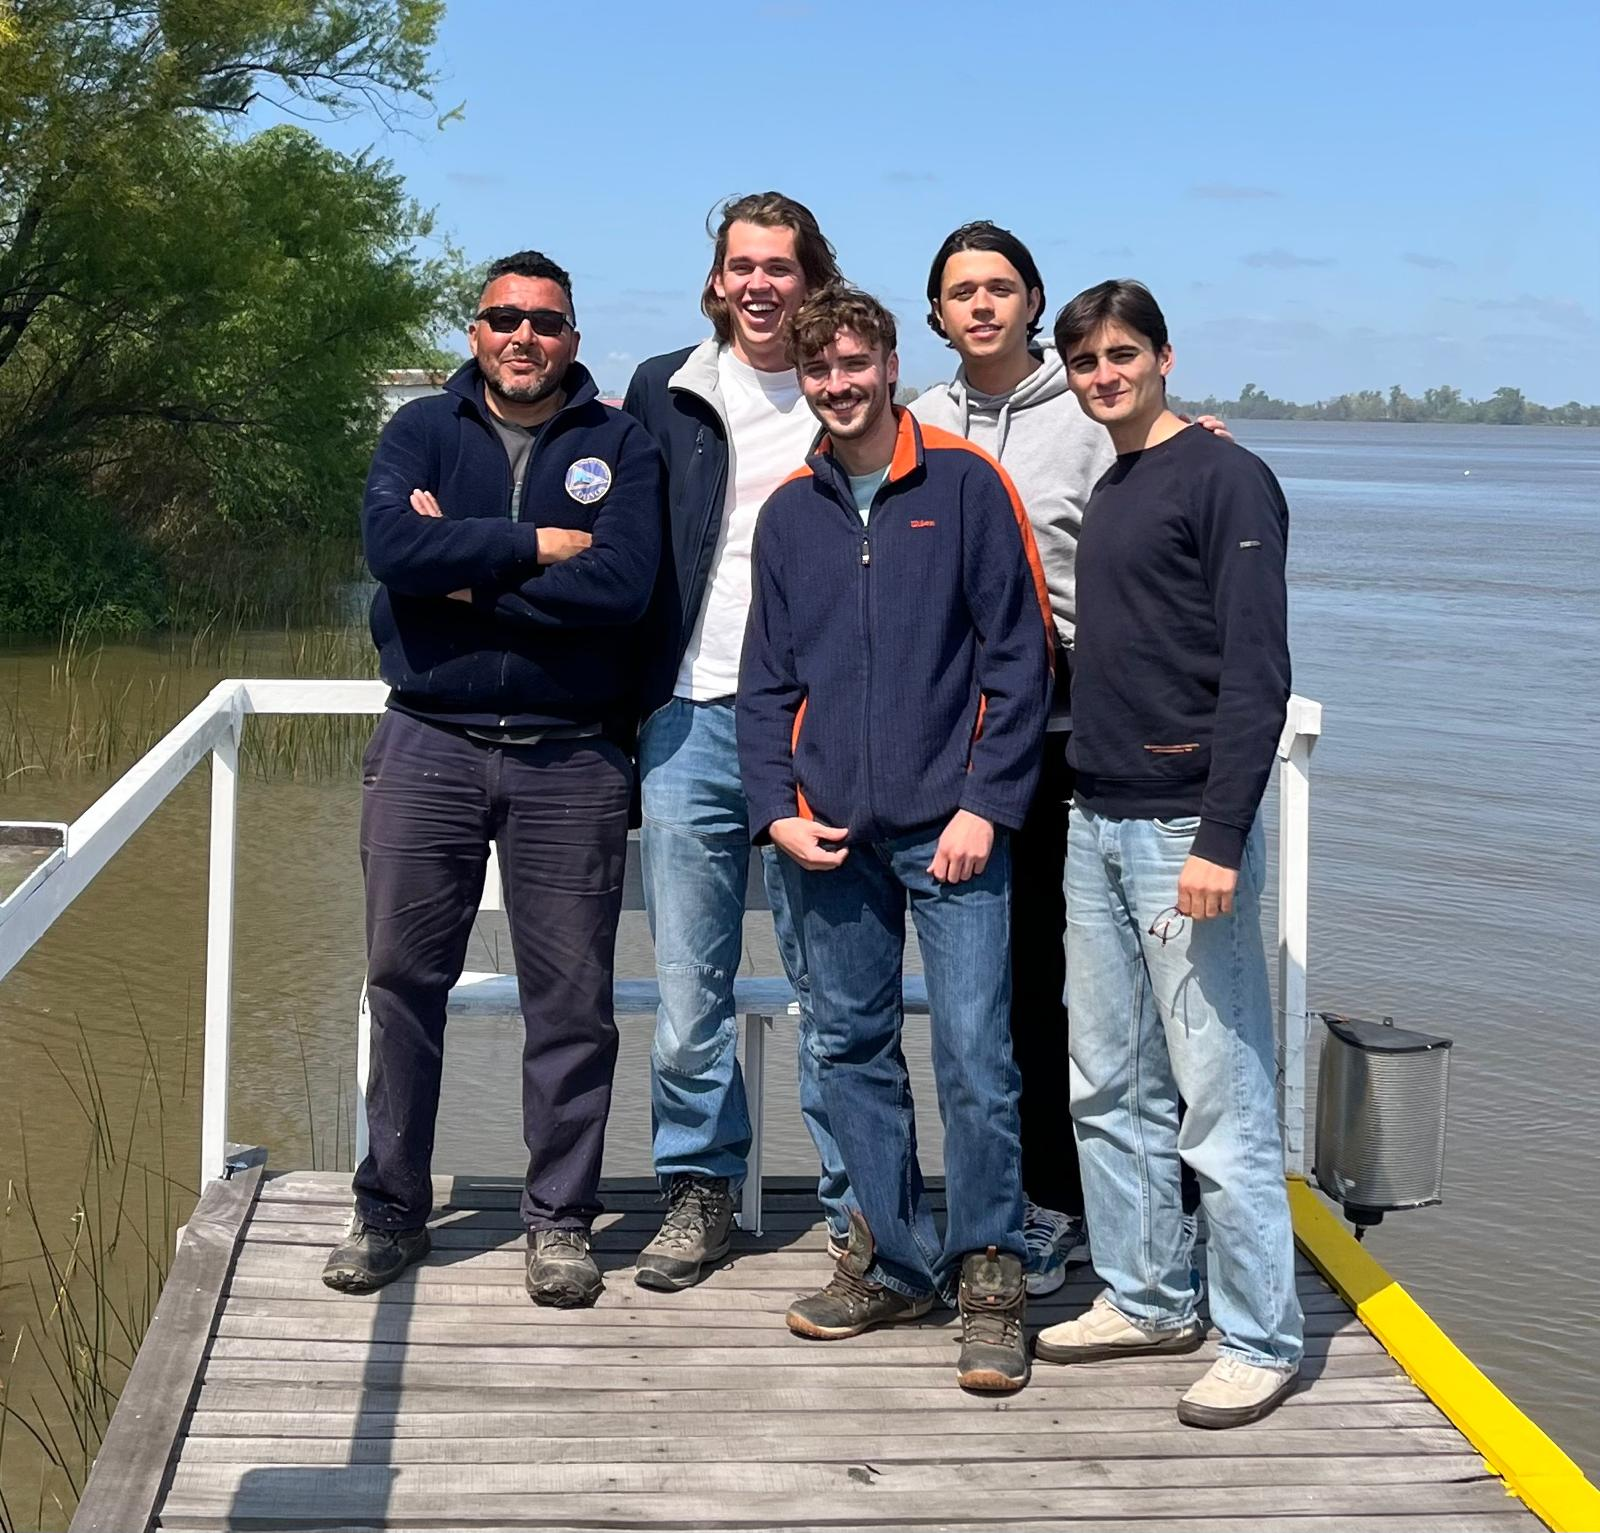
\includegraphics[width=0.4\linewidth]{figures/appendixE/InterviewFisher.jpeg}
\end{figure}

\textbf{Can you tell us something about the work you do in the Paraná Guazú?}
\begin{itemize}
    \item Club caretaker, responsible for maintenance of the club premises and receives members and guests.
\end{itemize}

\textbf{For how long have you been doing this job?}
\begin{itemize}
    \item Since 4.5 years.
\end{itemize}

\textbf{What are the changes you have seen over the years when it comes to the river and the fish in it?}
\begin{itemize}
    \item There is less fish than there was before.
    \item Some years ago: 1 person could catch 15 fish, recently there were 27 people who together caught 6 fish.
    \item This is due to contamination, fertilizers that are used on the land cause fish to die.
    \item When the water is low there is more fish than when the water is high. At the time of the interview the water was low, interviewee shows pictures of the entrance road that was fully flooded, now the water is meters lower. With high water, the water is dirtier.
\end{itemize}

\textbf{What kind of ships do you see on the water?}
\begin{itemize}
    \item He always sees 1 dredger boat, the name he doesn't recall.
    \item He sees 10 to 20 cargo ships going by per day.
\end{itemize}

\textbf{What do you know about sand mining in this region?}
\begin{itemize}
    \item The dry sand mining is the most important. Around 500 sand trucks per month leave the area, each truck carrying 40/45 tons. This number was half when he started his job 4.5 years ago.
    \item There used to be 9 sand companies, now 15.
    \item The dry sand miners work for YPF. It is used for fracking and they can only use the sand from here and Córdoba for that.
\end{itemize}

\textbf{Do you know anything about the dredging ships in particular?}
\begin{itemize}
    \item They used to bring sand to the port of Ibicuy, now not anymore.
    \item The sand from the river is yellow and muddy. It is used for construction.
\end{itemize}

\textbf{How many dredging ships do you see? Has this changed over the years? }
\begin{itemize}
    \item The same one has been dredging near the club for a long time, no increase seen.
    \item Only the dry sand mining activities have increased.
\end{itemize}

\textbf{Have you seen any damage to the river banks? Has this changed over the years?}
\begin{itemize}
    \item Yes, interviewee names a few examples.
    \item There was a collapse at the Ibicuy port 15 years ago.
    \item For the river banks: vegetation was removed near the club, this increased erosion.
\end{itemize}

\textbf{Results of unprepared questions:}
\begin{itemize}
    \item In the case of low water, ships sometimes get stuck upstream. Causes all ships to sail by at the same time, resulting in dirty water.
    \item A friend of the interviewee recently started a lawsuit because a dredger was operating in an illegal spot.
    \item Negative effects of dry sand mining: people complain because of the bad road conditions. The sand on the land absorbs water, so the mining has negative effects in case of floods. The sand is cleaned to get rid of organic parts, these parts flow back into the river. This makes the river dirty.
\end{itemize}

\section{Portmanager (Port of Puerto Ibicuy)}
\textbf{Name:} Matías \newline
\textbf{Role:} Port administrator \newline
\textbf{Date:} 24/9/2025 \newline
\textbf{Language of interview:} Spanish

\begin{figure}[H]
    \centering
    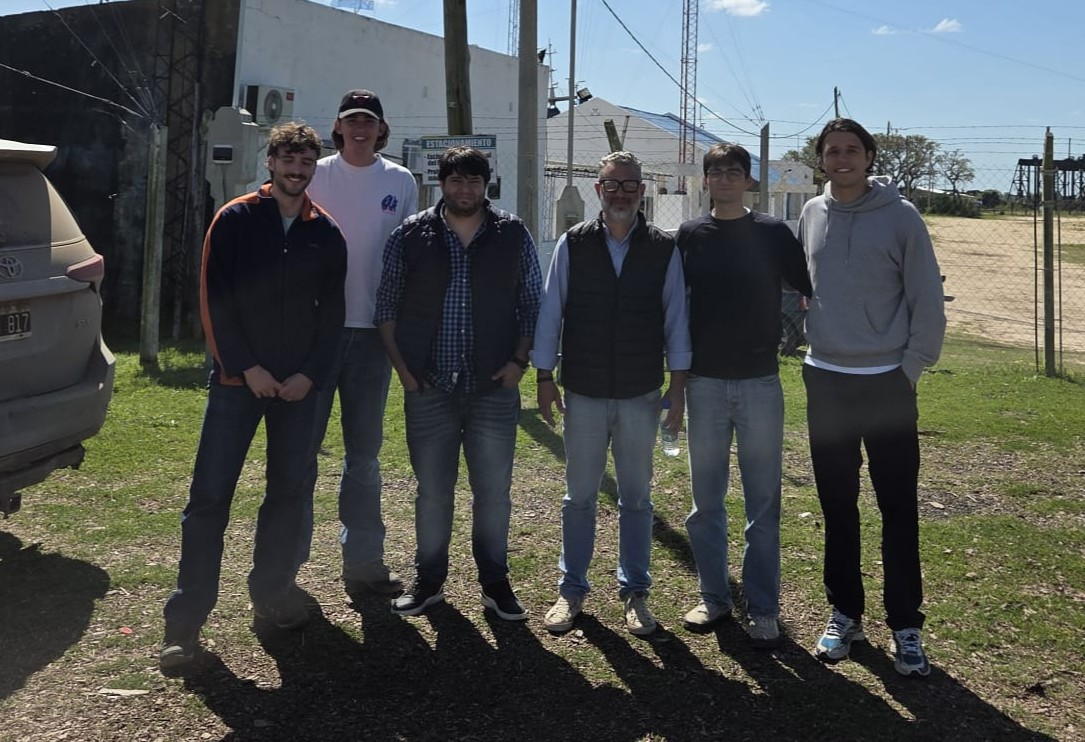
\includegraphics[width=0.5\linewidth]{figures/appendixE/InterviewPort.jpeg}
\end{figure}

\textbf{What kind of work do you do and for how long have you been in this position?}
\begin{itemize}
    \item Interviewee is the port administrator. He runs the port together with the port manager.
    \item Since 2020 in this position.
    \item The port manager changes after every local election and is appointed by the local government. Port administrator stays in place.
\end{itemize}

\textbf{Can you tell us something about the port and how it operates?}
\begin{itemize}
    \item Mostly wood is handled.
    \item They have two docks in the port, one of them is operating at the moment. Wood is handled there. The wood is used for construction and furniture purposes.
    \item Sometimes rice is handled.
    \item There were 19 ships in the port in 2024.
\end{itemize}

\textbf{How important is the handling of sand for the port?}
\begin{itemize}
    \item They used to handle sand from the dredgers, but not anymore.
    \item Sand is now handled by Puerto Constanza.
\end{itemize}

\textbf{How did the sand handling work? How much sand was it?}
\begin{itemize}
    \item It used to be small dredgers ships, of maximum 20 meters in length. There were two of these boats in the port. These ships are not active in the region anymore.
    \item They used pools to let the sand settle, water was flushed back in river.
    \item It was stopped because there were complaints about road conditions, a blame was needed.
    \item Interviewee does not know exact amounts of sand. The ships pay for the time at the dock, not for volumes.
\end{itemize}

\textbf{Did the sand mining activities increase over the last years?}
\begin{itemize}
    \item Since 2-3 years, there is more sand mining from the river.
    \item Upstream there is no sand mining activities and downstream there is a little.
    \item Since public construction projects were stopped by the government, the demand for sand is lower.
\end{itemize}

\textbf{Can you tell us something about the quay wall collapse that happened here?}
\begin{itemize}
    \item In 2011 the collapse happened.
    \item A ship left the dock, both ship and wall were heavily loaded. The water movement caused the failure of the wall.
    \item In 2016 it was restored.
    \item The dock was in good condition before the collapse.
\end{itemize}

\textbf{Results of unprepared questions:}
\begin{itemize}
    \item There is an illegal sand dump just North of the highway 12 bridge.
    \item The is a dry sand project that transports sand to Vaca Muerta. The dry sand mining is cheaper and high quality.
    \item The impacts of dredging are not because of mining activities but are due to maintenance of the channel. This does not happen on the Paraná-Ibicuy, but on the Paraná-Guazú river.
    \item Dredging boats get a permit per sector, there is always maximum 1 boat per zone.
\end{itemize}

\section{Plant manager (YPF sand mine)}
\textbf{Name:} Enzo \newline
\textbf{Role:} Plant manager \newline
\textbf{Date:} 26/9/2025 \newline
\textbf{Language of interview:} English

\begin{figure}[H]
    \centering
    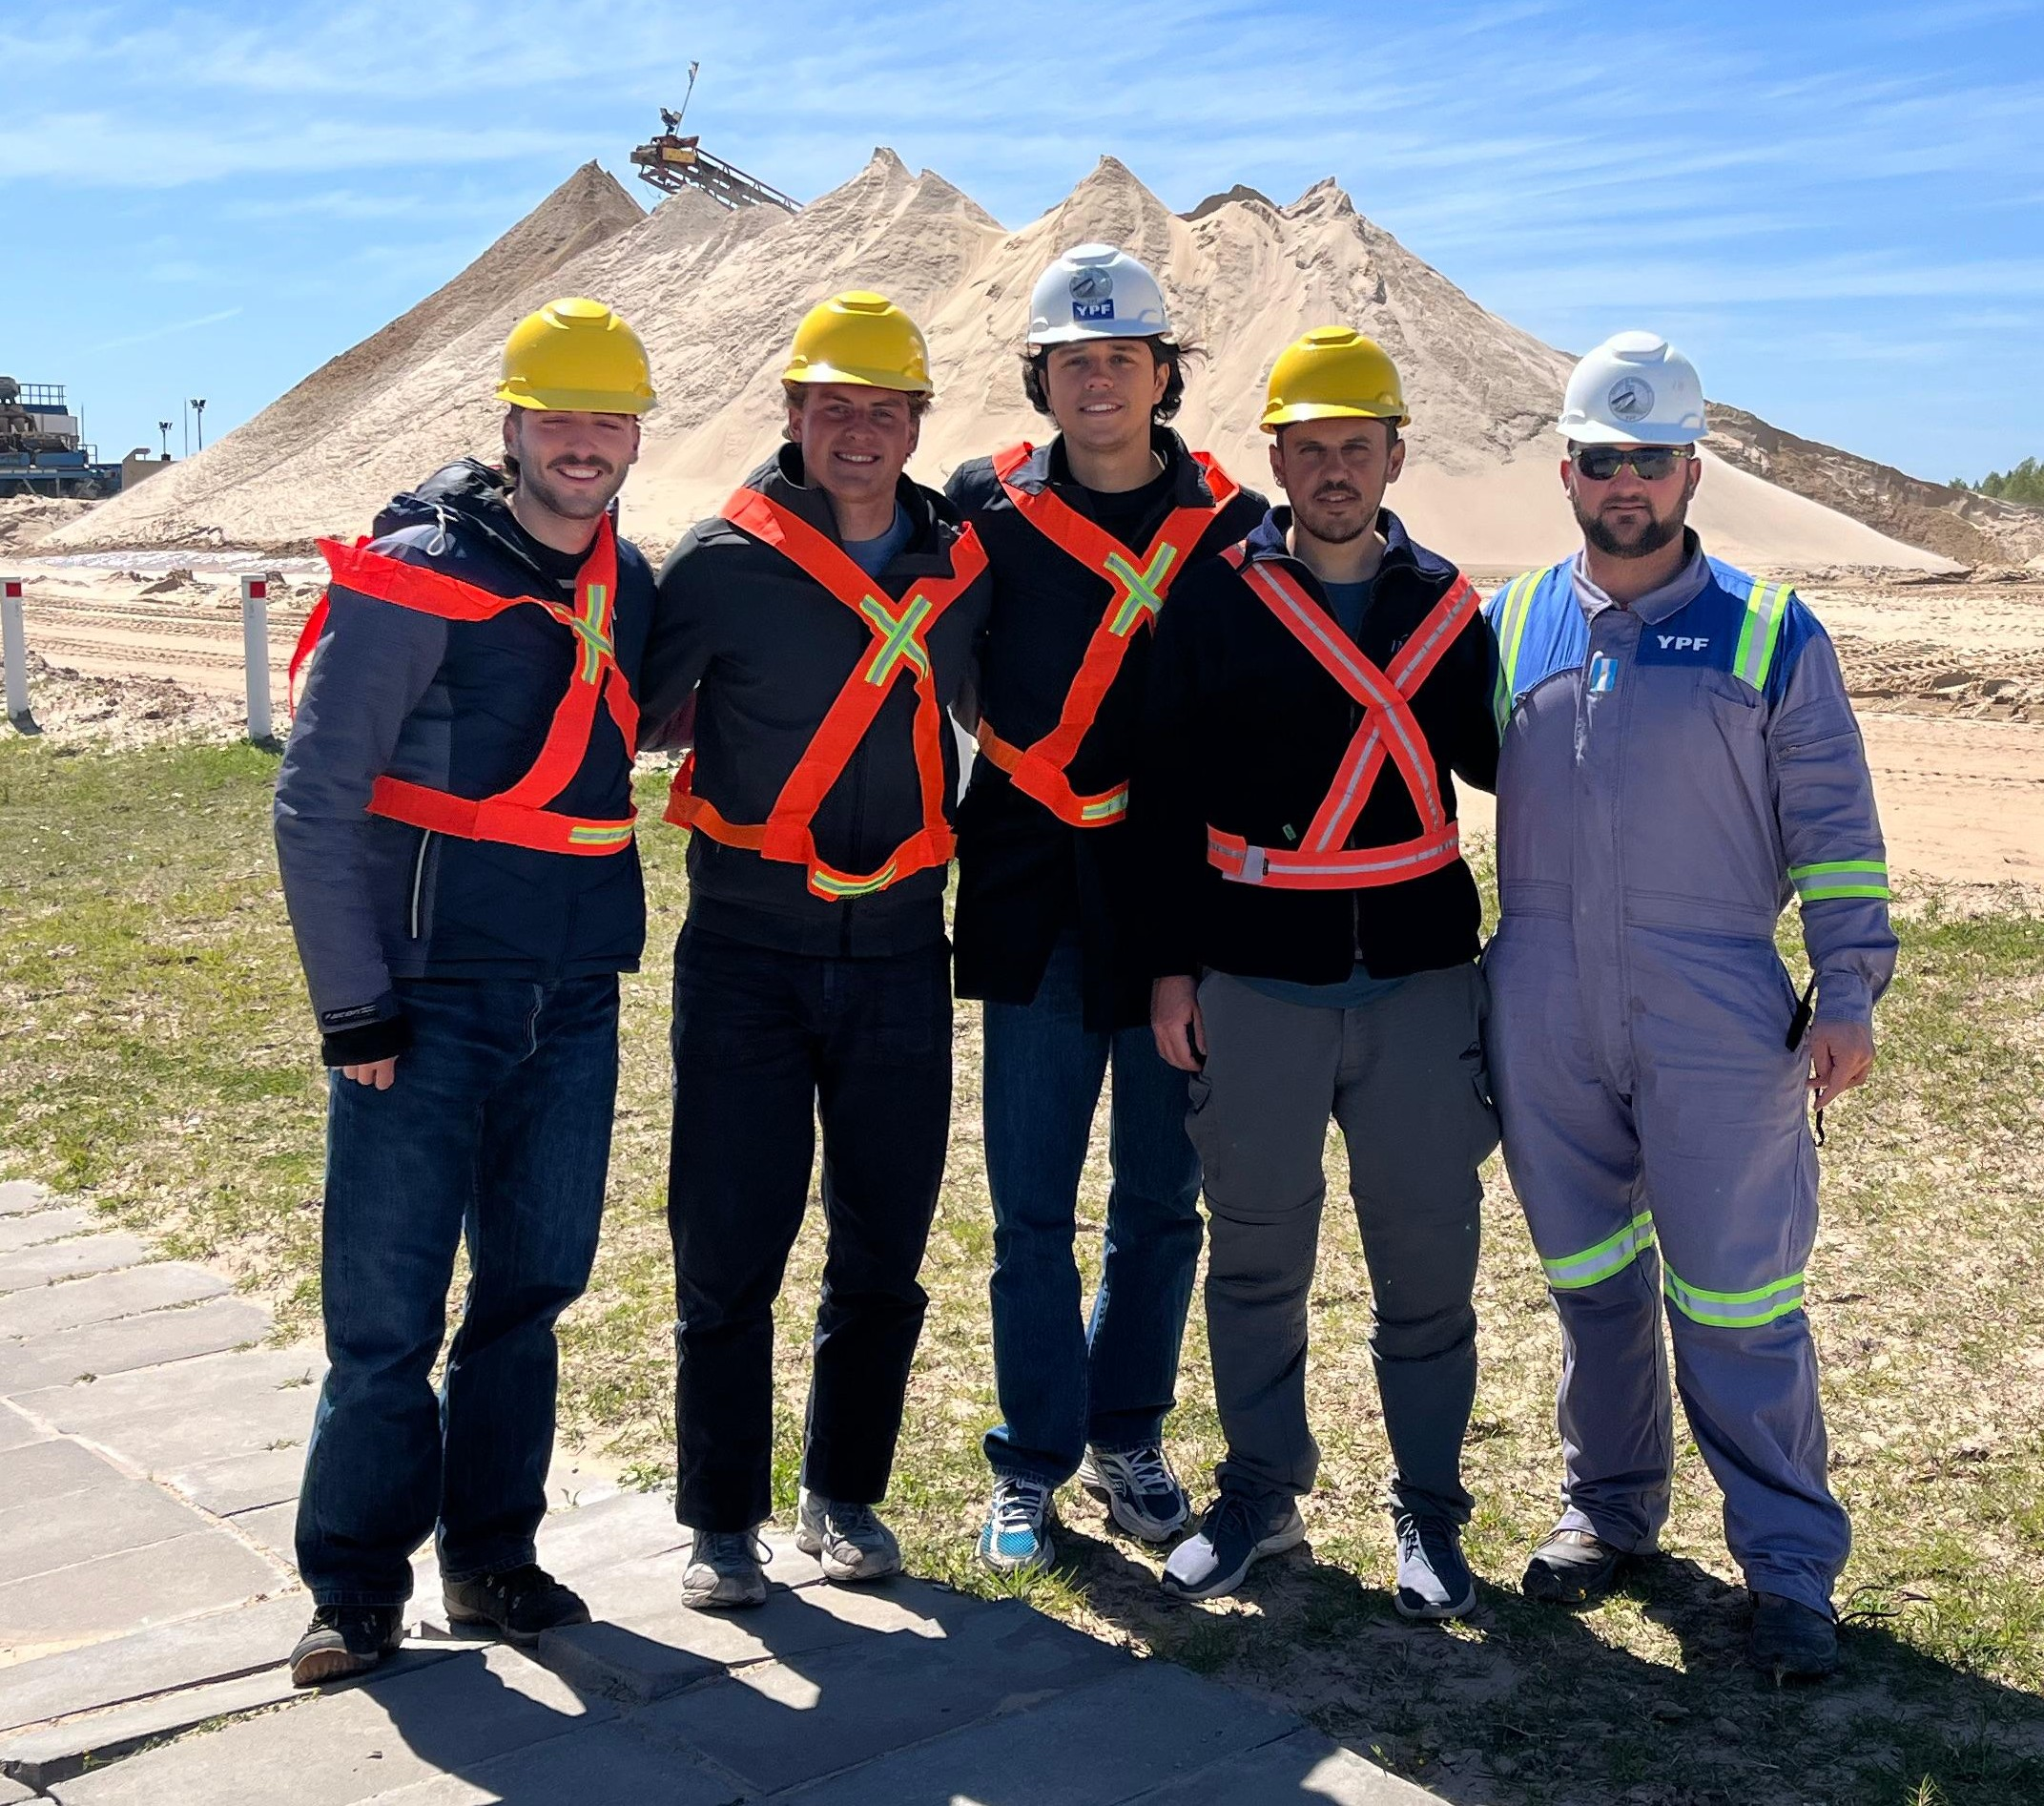
\includegraphics[width=0.4\linewidth]{figures/appendixE/InterviewYPF.jpeg}
\end{figure}

\textbf{Can you tell us something about the work you do?}
\begin{itemize}
    \item Interviewee is the boss of the quarry and is a geologist.
\end{itemize}

\textbf{How does the mine work?}
\begin{itemize}
    \item The plant is a sand mine. Sand is excavated and then washed to get the organic material out. Sand is put in tanks, through flocculation the clay parts are separated from the sand.
    \item The sand is used for fracking to mine shale oil and gas. The sand keeps the cracks open, so that the oil flows out.
    \item There are 70 people working at the mine.
\end{itemize}

\textbf{What are the characteristics of the soil here?}
\begin{itemize}
    \item There is a 5 m deep layer of fine sand. The median grane size is 0.1 mm. The sand here is uniquely fit for fracking.
    \item It consists for 99.875\% of quartz, which makes it a strong sand.
    \item Below the first sand layer, there is sometimes a clay layer of around 1 meter. This layer is locally concentrated and does not exist everywhere.
    \item Below this clay, there is more sand that can also be mined. Then there is another clay layer of between 6 to 10 m, gray in color. Finally, there is a thick, 30 to 40 m, sand layer with properties similar to river sand.
\end{itemize}

\textbf{What are the benefits of dry sand and sand from dredging?}
\begin{itemize}
    \item The river sand has a similar percentage of quartz.
    \item The sand from the land is more constant in size and the quality is therefore better.
    \item If the dredgers are organized better and if they buy a processing plant, it will be cheaper and good quality. Interviewee indicates that his plant would then lose to the competition.
\end{itemize}

\textbf{How much river sand is used by YPF?}
\begin{itemize}
    \item Around 30\% of sand used by YPF for fracking is from the river, the rest from the land.
    \item The biggest provided of river sand is located in San Pedro.
\end{itemize}

\textbf{How much sand do you mine? Is it more now than it was before?}
\begin{itemize}
    \item 120 thousand tons of sand is mined here each month.
    \item The demand for construction sand is low, but oil demand is high.
    \item Sand mining for fracking is a growing business.
    \item This mine can keep on operating for 8 to 10 years more, then the sand is gone. Study showed that there is 88 years of inland sand still available in the region.
    \item Next year, more sand will be mined than this year.
\end{itemize}

\textbf{Where does the sand go to?}
\begin{itemize}
    \item The sand goes to Añelo, the center of fracking in Argentina.
\end{itemize}

\textbf{How is the sand transported?}
\begin{itemize}
    \item Trucks are used. It takes 1 day to transport it to Añelo.
    \item There is an interest in moving to river transport. This is cheaper and the mine is located 200 m from the river.
    \item Due to limited availability and infrastructure problems, this is not yet realistic.
\end{itemize}

\textbf{Results of unprepared questions:}
\begin{itemize}
    \item The permits for dry sand mining hold for 3 years, then have to be renewed again. No amounts are specified in the permits, but taxes are paid per volume unit mined.
    \item The price for a cubic meter of sand is relatively constant if expressed in US Dollars.
    \item There are only a few locations in Argentina where sand for fracking is mined. In many places the characteristics and minerals are not fit for fracking. There are 6 mines in this region.
    \item An alternative to sand for fracking is not available or to be expected. Ceramic sand was used but was too expensive.
\end{itemize}

\section{Municipality of Zárate}
\textbf{Name:} Daniela \newline
\textbf{Role:} Municipality employee \newline
\textbf{Date:} 24/9/2025 \newline
\textbf{Language of interview:} Spanish \newline \newline
\textbf{Can you tell us something about the permits related to the dredging on the river?}
\begin{itemize}
    \item Interviewee indicates that she is not responsible for these permits. She shares contact details of colleagues that are involved in this.
    \item A new interview with these colleagues is planned for Friday 26/9/2025.
\end{itemize}

\textbf{Name:} Damian \newline
\textbf{Role:} Municipality employee \newline
\textbf{Date:} 26/9/2025 \newline
\textbf{Language of interview:} Spanish \newline \newline
\textbf{Can you tell us something about the permits related to the dredging on the river?}
\begin{itemize}
    \item Interviewee indicates that the permits are handled by the province, not the municipality.
\end{itemize}

\textbf{Do you know anything about a decrease in fish on the river?}
\begin{itemize}
    \item Fishers claim there is less fish, but this is due to a generational shift. She has not seen proof of there being less fish in the river.
\end{itemize}


\section{Mayor of Ibicuy}
\textbf{Name:} Ezequiel Maneiro \newline
\textbf{Role:} Mayor of the municipality of Ibicuy \newline
\textbf{Date:} 24/9/2025 \newline
\textbf{Language of interview:} Spanish \newline \newline

geen baggeren meer door toerisme, taxes hoger, bijna allemaal weg
alleen xx over

erosie is natuurlijk

constructie en glas

2 miljoen ton per jaar



\section{Landowners}
\textbf{Name:} Jorge and Marcelo \newline
\textbf{Role:} Owners of land next to the river \newline
\textbf{Date:} 24/9/2025 \newline
\textbf{Language of interview:} Spanish \newline \newline
\textbf{What is your experience with regard to the river?}
\begin{itemize}
    \item There is a lot of erosion. This is caused by big cargo ships and dredging boats.
    \item The erosion here is 30 m per year.
\end{itemize}

\textbf{Do you ever see dredging ships on the river?}
\begin{itemize}
    \item Yes, they know of two dredgers on the river.
    \item There used to be more dredgers on the river.
\end{itemize}

\textbf{What are the effects of dredging you see?}
\begin{itemize}
    \item The dredgers cause erosion and make the water dirty.
\end{itemize}

\section{Dredger}
\textbf{Name:} Daniel \newline
\textbf{Role:} Sand miner on the river\newline
\textbf{Date:} 25/9/2025 \newline
\textbf{Language of interview:} Spanish \newline \newline
\textbf{Can you tell us something about the work you do in the Parana Guazu?}
\begin{itemize}
    \item I am the owner of the ship and this port. At the moment we are making the port ready to start with our sand mining activities. With a small cutter we are dredging out our harbour and I am replacing some parts in my ship. 
    \item If we start operating we will do two trips a day. 
\end{itemize}

\textbf{For how long have you been doing this job?}
\begin{itemize}
    \item We went to this location 2 years ago.
    \item Before that I have been working for 3 years to get the permits. Getting the permits was a lot of work. The government is extremely slow. 
    \item Before this place, we have dredged at a different location
    \item You need to get permission from three different parties, the prefectura, the municipality and the county. 
\end{itemize}

\textbf{Are you operating by yourself or are you working for an organization?}
\begin{itemize}
    \item I am a private entrepreneur.  
\end{itemize}

\textbf{Do you do this work every day, throughout the whole year?}
\begin{itemize}
    \item Every normal day we work here. (not on the weekends and special days)
\end{itemize}

\textbf{Can you walk us through your regular work day?}
\begin{itemize}
    \item When we are fully operating, we go mining twice a day and about 20 trucks come to us to get sand. at the entrance of our harbour is a weighing bridge where we weigh how much sand the truck takes with him.
\end{itemize}

\textbf{How much sand can your ship carry?}
\begin{itemize}
    \item Around 600 cubic meters of sand. 
\end{itemize}

\textbf{Where do you leave the sand after mining it?}\usepackage
\begin{itemize}
    \item After mining the ship will travel back to our harbour. There, it will mix the sand with water and pump it through a pipe to a big field which is surrounded with dikes and a channel.
    \item The channel is used to get the water back in the river.
    \item From this place is the sand transported with trucks to buyers.
\end{itemize}

\textbf{What happens with the sand after you leave it there?}
\begin{itemize}
    \item The sand is mostly used for construction works (mostly concrete)
    \item The demand for sand for construction works has dramatically reduced because of government policy, so now we also sell sand to be used in the cracking process. 
    \item For the cracking process must the sand be very small grained. 
\end{itemize}

\textbf{Can you tell something about the ship you are using?}
\begin{itemize}
    \item Yes of course!! I can also show you the ship if you want. 
    \item The ship is called the Vizcaino 978, she is build in the 50's. The ship has always been used for sand mining. I bought her a few years ago. 
    \item Trough a pipe is the sand sucked from the riverbed. This is done with an hydraulic pump. then it goes to the highest point, in this point is some of the material poured back into the river because its to fine material (clay and silt). 
    \item the sand goes from this point over a slide. On the slide the workers on the ship can open several entrances from which it falls into the sand storage. This continues till the storage is full
    \item Then the ship will sail back to the port and mix the sand with water where this slurry is pumped to the shore. 
\end{itemize}

\textbf{How is the price of sand at the moment?}
\begin{itemize}
    \item The price of sand for construction works has been quite constant true the years (not talking about the inflation differences), but the demand has been less and less.
    \item The price of sand for cracking has more fluctuations but the demand is always quite high.
\end{itemize}

